% CH4114 --- Tutorial 00, Part 4: NumPy & Matplotlib
% Beamer deck, 16:9, compiled with pdflatex (TeX Live 2026)
% Author: Shuvam Banerji Seal
\documentclass[aspectratio=169]{beamer}

\usetheme{Madrid}
\usecolortheme{whale}
\setbeamertemplate{navigation symbols}{}

\usepackage[T1]{fontenc}
\usepackage{tikz}
\usetikzlibrary{arrows.meta, positioning}
\usepackage{booktabs}
\usepackage{listings}
\lstset{
  basicstyle=\ttfamily\footnotesize,
  breaklines=true,
  showstringspaces=false,
  columns=fullflexible,
  keepspaces=true,
}

\title[NumPy \& Matplotlib]{Tutorial 00 --- Part 4\\[2pt] NumPy \& Matplotlib}
\subtitle{Arrays, random numbers, and plots}
\author[SBS]{Shuvam Banerji Seal}
\institute[CH4114]{CH4114 --- Molecular Simulation}
\date[Aug 2026]{14 August 2026}

\begin{document}

% ------------------------------------------------------------------ title
\begin{frame}[plain]
  \titlepage
  \centering{\scriptsize Course Instructor: Dr.\ Susmita Roy \quad$\cdot$\quad TA: Shuvam Banerji Seal}\par
  \vspace{0.1cm}
  \centering{\scriptsize Repository: \texttt{CH4114\_Molecular\_Simulation\_Tutorials}}
\end{frame}

% ------------------------------------------------------------ two pillars
\begin{frame}{The two pillars of scientific Python}
  \begin{center}
    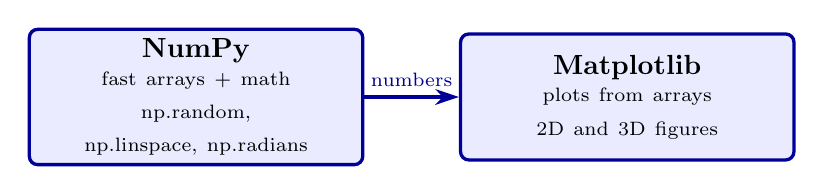
\begin{tikzpicture}[
        p/.style={rectangle, draw=blue!60!black, very thick, rounded corners=3pt,
                  fill=blue!8, text width=4.0cm, align=center, minimum height=1.6cm},
        arr/.style={-{Stealth[length=3mm,width=2mm]}, very thick, blue!60!black},
        node distance=1.2cm]
      \node[p] (np) {\textbf{NumPy}\\[2pt] {\scriptsize fast arrays + math\\ np.random, np.linspace, np.radians}};
      \node[p, right=of np] (mp) {\textbf{Matplotlib}\\[2pt] {\scriptsize plots from arrays\\ 2D and 3D figures}};
      \draw[arr] (np) -- node[above, font=\scriptsize] {numbers} (mp);
    \end{tikzpicture}
  \end{center}
  \begin{itemize}
    \item Every simulation this semester is built on NumPy arrays.
    \item Every result is understood through a Matplotlib figure.
  \end{itemize}
  \begin{block}{The standard imports}
    \texttt{import numpy as np} \quad\quad \texttt{import matplotlib.pyplot as plt}
  \end{block}
\end{frame}

% ---------------------------------------------------------------- arrays
\begin{frame}[fragile]{NumPy arrays --- the basic container}
  \begin{columns}[T]
    \begin{column}{0.48\textwidth}
      \begin{lstlisting}
a = np.array([1, 2, 3, 4, 5])
a.shape      # (5,)
a.dtype      # int64
a[0]         # 1
a[-1]        # 5
a[1:4]       # [2 3 4]

m = np.array([[1, 2], [3, 4]])
m.shape      # (2, 2)
m[0, 1]      # 2
      \end{lstlisting}
    \end{column}
    \begin{column}{0.48\textwidth}
      \begin{itemize}
        \item An array is like a list, but \textbf{fast and math-aware}.
        \item \texttt{shape} = size per dimension.
        \item \texttt{dtype} = type of the elements.
        \item Indexing and slicing work exactly like lists.
      \end{itemize}
    \end{column}
  \end{columns}
\end{frame}

% ------------------------------------------------------------ big five
\begin{frame}{The big five array creators}
  \begin{table}
    \small
    \begin{tabular}{@{}ll@{}}
      \toprule
      Function & What it does \\
      \midrule
      \texttt{np.array([...])} & array from a Python list \\
      \texttt{np.arange(a, b, s)} & evenly spaced \emph{integers} \\
      \texttt{np.linspace(a, b, n)} & \textbf{n} evenly spaced values, inclusive \\
      \texttt{np.zeros(s)} / \texttt{np.ones(s)} & array filled with 0 or 1 \\
      \texttt{np.zeros\_like(x)} & zeros with the same shape as \texttt{x} \\
      \bottomrule
    \end{tabular}
  \end{table}
  \vspace{0.3cm}
  \begin{alertblock}{\texttt{np.linspace} is the most-used NumPy function in this course}
    \texttt{x = np.linspace(0, 2*np.pi, 100)} --- the x-values of every plot you will make.
  \end{alertblock}
\end{frame}

% ---------------------------------------------------------------- random
\begin{frame}{Random numbers: np.random}
  \begin{table}
    \small
    \begin{tabular}{@{}ll@{}}
      \toprule
      Function & What it gives you \\
      \midrule
      \texttt{np.random.rand(n)} & n values uniform in [0, 1) \\
      \texttt{np.random.randint(a, b, n)} & n random integers in [a, b) \\
      \texttt{np.random.normal(m, s, n)} & n Gaussian values \\
      \texttt{np.random.uniform(a, b, n)} & n values uniform in [a, b) \\
      \texttt{np.random.choice(x, n)} & n random picks from x \\
      \bottomrule
    \end{tabular}
  \end{table}
  \vspace{0.3cm}
  \begin{alertblock}{Always set the seed first}
    \texttt{np.random.seed(42)} --- makes ``random'' results \textbf{reproducible}.
    This is the heart of Monte Carlo simulation.
  \end{alertblock}
\end{frame}

% ---------------------------------------------------------------- angles
\begin{frame}{Angles: np.radians and np.degrees}
  \begin{center}
    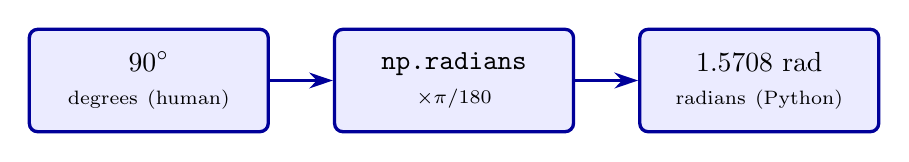
\begin{tikzpicture}[
        b/.style={rectangle, draw=blue!60!black, very thick, rounded corners=3pt,
                  fill=blue!8, text width=2.8cm, align=center, minimum height=1.3cm},
        arr/.style={-{Stealth[length=3mm,width=2mm]}, very thick, blue!60!black},
        node distance=0.8cm]
      \node[b] (d) {$90^\circ$ \\ {\scriptsize degrees (human)}};
      \node[b, right=of d] (r) {\texttt{np.radians} \\ {\scriptsize $\times \pi/180$}};
      \node[b, right=of r] (rd) {1.5708 rad \\ {\scriptsize radians (Python)}};
      \draw[arr] (d) -- (r);
      \draw[arr] (r) -- (rd);
    \end{tikzpicture}
  \end{center}
  \vspace{0.3cm}
  \begin{itemize}
    \item \texttt{np.sin}, \texttt{np.cos}, \texttt{np.tan} expect \textbf{radians}.
    \item \texttt{np.degrees(rad)} converts back.
    \item Useful constants: \texttt{np.pi}, \texttt{np.sqrt}, \texttt{np.exp}, \texttt{np.abs}.
  \end{itemize}
\end{frame}

% ------------------------------------------------------------ elementwise
\begin{frame}[fragile]{Math on arrays --- no loops needed}
  \begin{block}{The Lennard-Jones potential (you will use this pattern constantly)}
    \begin{lstlisting}
r = np.linspace(0.3, 1.0, 50)     # 50 distances in nm
sigma, epsilon = 0.34, 0.997      # LJ parameters
sr = sigma / r                    # divide EVERY element by r
lj = 4 * epsilon * (sr**12 - sr**6)   # formula on the whole array
lj.min(), lj.mean(), lj.sum()     # quick statistics
    \end{lstlisting}
  \end{block}
  \begin{itemize}
    \item Generate a range with \texttt{linspace}, apply a formula, get an array back.
    \item This is exactly how simulation analysis code is written.
  \end{itemize}
\end{frame}

% ------------------------------------------------------------- first plot
\begin{frame}[fragile]{Matplotlib --- your first 2D plot}
  \begin{center}
    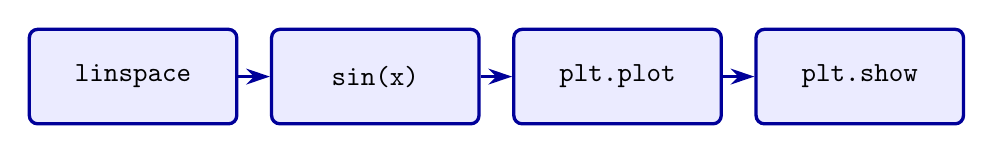
\begin{tikzpicture}[
        b/.style={rectangle, draw=blue!60!black, very thick, rounded corners=3pt,
                  fill=blue!8, text width=2.4cm, align=center, minimum height=1.2cm},
        arr/.style={-{Stealth[length=3mm,width=2mm]}, very thick, blue!60!black},
        node distance=0.4cm]
      \node[b] (a) {\texttt{linspace}};
      \node[b, right=of a] (b) {\texttt{sin(x)}};
      \node[b, right=of b] (c) {\texttt{plt.plot}};
      \node[b, right=of c] (d) {\texttt{plt.show}};
      \draw[arr] (a) -- (b);
      \draw[arr] (b) -- (c);
      \draw[arr] (c) -- (d);
    \end{tikzpicture}
  \end{center}
  \begin{lstlisting}
x = np.linspace(0, 2*np.pi, 100)
y = np.sin(x)
plt.plot(x, y)
plt.title("Sine wave"); plt.xlabel("angle (rad)"); plt.ylabel("sin(x)")
plt.grid(True); plt.show()
  \end{lstlisting}
\end{frame}

% --------------------------------------------------------------- colors
\begin{frame}[fragile]{Colors, styles, and legends}
  \begin{table}
    \small
    \begin{tabular}{@{}ll@{}}
      \toprule
      Color ways & Examples \\
      \midrule
      named color & \texttt{"red"}, \texttt{"crimson"}, \texttt{"forestgreen"} \\
      hex code & \texttt{"\#2E86AB"}, \texttt{"\#FF5733"} \\
      RGB tuple & \texttt{(0.1, 0.4, 0.9)} \\
      single letter & \texttt{'r'}, \texttt{'g'}, \texttt{'b'}, \texttt{'k'} \\
      \bottomrule
    \end{tabular}
  \end{table}
  \vspace{0.3cm}
  \begin{lstlisting}
plt.plot(x, np.sin(x), color="crimson", label="sin")
plt.plot(x, np.cos(x), color="#2E86AB", linestyle="--", label="cos")
plt.scatter(x[::10], np.sin(x[::10]), color="green", s=30)
plt.legend()     # shows the labels
  \end{lstlisting}
\end{frame}

% ------------------------------------------------------------- subplots
\begin{frame}[fragile]{Subplots --- several panels in one figure}
  \begin{columns}[T]
    \begin{column}{0.48\textwidth}
      \begin{lstlisting}
fig, axes = plt.subplots(1, 2,
                         figsize=(10, 4))
axes[0].plot(x, np.sin(x))
axes[0].set_title("sin")
axes[1].plot(x, np.cos(x))
axes[1].set_title("cos")
plt.tight_layout()
plt.show()
      \end{lstlisting}
    \end{column}
    \begin{column}{0.48\textwidth}
      \begin{itemize}
        \item \texttt{subplots(rows, cols)} returns a figure and axes.
        \item Draw on each axes: \texttt{axes[0].plot(...)}.
        \item Inside an axes use \texttt{set\_title}, \texttt{set\_xlabel}.
        \item Grid: \texttt{subplots(2, 2)} $\rightarrow$ \texttt{axes[0,0]}, \texttt{axes[0,1]}, \ldots
      \end{itemize}
    \end{column}
  \end{columns}
\end{frame}

% -------------------------------------------------------------- surface
\begin{frame}[fragile]{3D surface plots}
  \begin{center}
    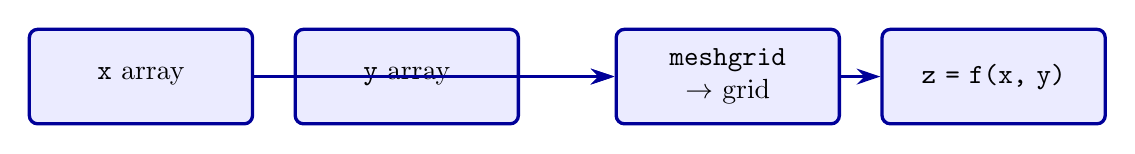
\begin{tikzpicture}[
        b/.style={rectangle, draw=blue!60!black, very thick, rounded corners=3pt,
                  fill=blue!8, text width=2.6cm, align=center, minimum height=1.2cm},
        arr/.style={-{Stealth[length=3mm,width=2mm]}, very thick, blue!60!black},
        node distance=0.5cm]
      \node[b] (x) {\texttt{x} array};
      \node[b, right=of x] (y) {\texttt{y} array};
      \node[b, right=1.2cm of y] (g) {\texttt{meshgrid} $\rightarrow$ grid};
      \node[b, right=of g] (z) {\texttt{z = f(x, y)}};
      \draw[arr] (x) -- (g);
      \draw[arr] (y) -- (g);
      \draw[arr] (g) -- (z);
    \end{tikzpicture}
  \end{center}
  \begin{lstlisting}
ax = fig.add_subplot(111, projection="3d")
X, Y = np.meshgrid(u, u)               # grid of (x, y) pairs
Z = np.exp(-(X**2 + Y**2))             # value at every grid point
ax.plot_surface(X, Y, Z, cmap="viridis")   # colored surface
  \end{lstlisting}
  \begin{itemize}
    \item Colormaps: \texttt{"viridis"}, \texttt{"plasma"}, \texttt{"coolwarm"}, \texttt{"magma"}.
  \end{itemize}
\end{frame}

% --------------------------------------------------------------- rotate
\begin{frame}[fragile]{3D scatter and rotating with your mouse}
  \begin{columns}[T]
    \begin{column}{0.48\textwidth}
      \begin{lstlisting}
np.random.seed(7)
n = 50
xs = np.random.rand(n)
ys = np.random.rand(n)
zs = np.random.rand(n)
ax.scatter(xs, ys, zs,
           s=50, c=zs, cmap="plasma")
      \end{lstlisting}
    \end{column}
    \begin{column}{0.48\textwidth}
      \begin{block}{Mouse controls (any 3D plot)}
        \begin{itemize}
          \item \textbf{Drag} left button $\rightarrow$ rotate
          \item \textbf{Right-drag} $\rightarrow$ zoom
          \item \textbf{Scroll} $\rightarrow$ zoom in/out
        \end{itemize}
      \end{block}
      \begin{itemize}
        \item Script: \texttt{plt.show()} opens a rotatable window.
        \item Jupyter: \texttt{\%matplotlib widget} (needs \texttt{ipympl}).
      \end{itemize}
    \end{column}
  \end{columns}
\end{frame}

% --------------------------------------------------------------- summary
\begin{frame}[fragile]{Scripts, notebooks, and check yourself}
  \begin{block}{Run the companion code}
    \begin{lstlisting}
uv run python examples/numpy_matplotlib/numpy_basics.py
uv run python examples/numpy_matplotlib/matplotlib_plots.py
    \end{lstlisting}
  \end{block}
  \begin{block}{Check yourself}
    \begin{enumerate}
      \item \texttt{np.arange(0,10,2)} vs \texttt{np.linspace(0,10,2)} --- difference?
      \item Why set \texttt{np.random.seed(...)} before using \texttt{np.random}?
      \item Which function converts degrees to radians? Why is it needed for \texttt{np.sin}?
      \item What does \texttt{np.zeros\_like(x)} return?
      \item How do you make a 1$\times$3 grid of subplots? A 3D axes?
    \end{enumerate}
  \end{block}
\end{frame}

\end{document}